%%% CV de Romain REIGNIER créé grâce au template suivant :

%%% LaTeX Template: Designer's CV
%%%
%%% Source: http://www.howtotex.com/
%%% Feel free to distribute this template, but please keep the referal to HowToTeX.com.
%%% Date: March 2012

%%%%%%%%%%%%%%%%%%%%%%%%%%%%%%%%%%%%%
% Document properties and packages
%%%%%%%%%%%%%%%%%%%%%%%%%%%%%%%%%%%%%
\documentclass[a4paper,11pt,final]{memoir}

% misc
\renewcommand{\familydefault}{bch} % font
\pagestyle{empty}					         % no pagenumbering
\setlength{\parindent}{0pt}			   % no paragraph indentation

\usepackage[T1]{fontenc}
\usepackage[utf8]{inputenc}
% required packages (add your own)
\usepackage{flowfram}										 % column layout
\usepackage[top=1cm,left=1cm,right=1cm,bottom=1cm]{geometry}% margins
\usepackage{graphicx}										 % figures
\usepackage{url}											   % URLs
\usepackage[usenames,dvipsnames]{xcolor} % color
\usepackage{multicol}										 % columns env.
	\setlength{\multicolsep}{0pt}
\usepackage{paralist}										 % compact lists
\usepackage{tikz}
\usepackage{hyperref}
\hypersetup{colorlinks,citecolor=black,filecolor=black,linkcolor=black,urlcolor=black} % pour mettre les liens en noirs, sans cadre
\usepackage[francais]{babel}

\definecolor{dark_gray}{rgb}{0.3,0.3,0.3}

%%%%%%%%%%%%%%%%%%%%%%%%%%%%%%%%%%%%%
% Create column layout
%%%%%%%%%%%%%%%%%%%%%%%%%%%%%%%%%%%%%
% define length commands
\setlength{\vcolumnsep}{\baselineskip}
\setlength{\columnsep}{\vcolumnsep}

% frame setup (flowfram package)
% left frame
\newflowframe{0.27\textwidth}{\textheight}{0pt}{0pt}[left]
	\newlength{\LeftMainSep}
	\setlength{\LeftMainSep}{0.26\textwidth}
	\addtolength{\LeftMainSep}{1\columnsep}

% small static frame for the vertical line
\newstaticframe{1.5pt}{\textheight}{\LeftMainSep}{0pt}

% content of the static frame
\begin{staticcontents}{1}
\hfill
\tikz{%
	\draw[loosely dotted,color=RoyalBlue,line width=1.5pt,yshift=0]
	(0,0) -- (0,\textheight);}%
\hfill\mbox{}
\end{staticcontents}

% right frame
\addtolength{\LeftMainSep}{1.5pt}
\addtolength{\LeftMainSep}{1\columnsep}
\newflowframe{0.68\textwidth}{\textheight}{\LeftMainSep}{0pt}[main01]

%%%%%%%%%%%%%%%%%%%%%%%%%%%%%%%%%%%%%
% define macros (for convience)
%%%%%%%%%%%%%%%%%%%%%%%%%%%%%%%%%%%%%
\newcommand{\Sep}{\vspace{1.3em}}
\newcommand{\SmallSep}{\vspace{0.5em}}

\newenvironment{AboutMe}
	{\ignorespaces}%\textbf{\color{RoyalBlue} About me}}
	{\SmallSep\ignorespacesafterend}

\newcommand{\CVSection}[1]
	{\Large\textbf{#1}\par
	\SmallSep\normalsize\normalfont}

\newcommand{\CVItem}[2]
	{\textbf{\color{RoyalBlue} #1 \color{dark_gray} #2}\normalsize\normalfont}

\newcommand{\city}[1]
	{{\small\color{dark_gray}\emph{#1}}\normalsize\normalfont}

\newcommand{\SkillSection}[1]
	{\normalsize{\textbf{#1\\}}\normalfont\small}%\footnotesize}

\newcommand{\SkillItem}[1]
{\vspace{0.25em}\textbf{\color{RoyalBlue} #1}\normalfont}

%%%%%%%%%%%%%%%%%%%%%%%%%%%%%%%%%%%%%
% Begin document
%%%%%%%%%%%%%%%%%%%%%%%%%%%%%%%%%%%%%
\begin{document}

% Left frame
%%%%%%%%%%%%%%%%%%%%
% Photo
\begin{figure}
	\hfill
	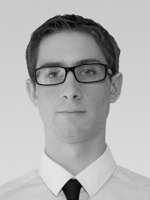
\includegraphics[width=0.5\columnwidth]{../IMG_7936-Modifier_cv}
	\vspace{-0.5cm}
\end{figure}

% Personnal Infos
\begin{flushright}\small
	%Romain \textsc{Reignier} \\
	83 avenue du Général Leclerc\\
	33200 Bordeaux\\
	%France\\
	{\href{mailto:rom.reignier@gmail.com}{\nolinkurl{rom.reignier@gmail.com}}}\\
	06 09 52 16 18\\
	24 ans\\
	Permis B
\end{flushright}%\normalsize

\begin{flushleft}
% Engineering
\SkillSection{Compétences}
Conception mécanique\\
CAO \& CFAO\\
%Résistance des matériaux\\
Électronique\\
Conception de systèmes\\
%Analyse des mécanismes\\
%Materials\\
Méthodes numériques\\
%Algorithmique\\
%Database\\
%Thermal transferts\\
Automatique\\
%Systèmes asservis\\
Robotique\\
%Communication\\
%Vison par ordinateur\\
Traitement d'image
\SmallSep

% Computer Skills
\SkillSection{Informatique}
\vspace{-0.25em}
\SkillItem{Programmation}\\
%\verb!C!, \verb!C++!, Python, Matlab/Simulink, LabView, Java, OpenCV, Qt\\ %Maple
	C, \textbf{C++}, \textbf{Python}, Matlab/Simulink, LabView, OpenCV, \textbf{Qt}, Git, CI\\ %Maple
\SkillItem{Robotique}\\
\textbf{Robot Operating System} (ROS), \textbf{Gazebo}\\
\SkillItem{Embarqué}\\
GNU/Linux (Raspberry Pi, BBB), Microcontôleurs (Arduino, AVR, dsPIC, STM32)\\%, assembleur ST8\\
\SkillItem{CAO}\\
CATIA V5, SolidWorks\\
\SkillItem{Développement Web}\\
JQuery, Bootstrap\\
%\SkillItem{Bureautique}\\
%Word, Excel (Visual Basic), PowerPoint, Access, Project, \LaTeX
%%\SkillItem{Graphisme}\\
%%Photoshop, Lightroom, Illustrator, Gimp, Inkscape, FinalCut Pro X\\
\SmallSep

% Languages
\SkillSection{Langues}
\vspace{-0.25em}
\SkillItem{Anglais} : Écrit et parlé\\%(TOEIC : 920 pts)\\
\SkillItem{Espagnol} : Niveau Baccalauréat\\
\SkillItem{Allemand} : Notions
\SmallSep

% Sports
\SkillSection{Sports}
Cyclisme (4 ans en compétition)\\
VTT\\
Course à pied\\
%Swimming
\SmallSep

% Hobbies
%\SkillSection{Loisirs}
\SkillSection{Passions}
Robotique\\
Mécanique\\
Machinisme Agricole\\
%Agriculture\\
Photographie\\
Brevet d'Initiation à l'Aéronautique
\SmallSep

% Travels
\SkillSection{Voyages}
Malaisie, Singapour,\\Togo (humanitaire),\\
InterRail 2014 : Amsterdam, Berlin, Prague, Vienne, Genève
%Pays-Bas, Allemagne, République Tchèque, Autriche, Suisse
\end{flushleft}
\framebreak

% Right frame
%%%%%%%%%%%%%%%%%%%%
%\Huge\bfseries {\color{RoyalBlue} Romain \textsc{Reignier}} \\
\Huge\bfseries {\color{RoyalBlue} Romain REIGNIER} \\
\Large\bfseries  Ingénieur Supméca Mécatronique et Robotique\\
% About
%\begin{AboutMe}
%\end{AboutMe}


% Experience
\CVSection{Expériences}
\CVItem{Janvier 2016 -- Octobre 2016,}{INRIA et Génération Robots} -- \city{Bordeaux}\\
Développement d'un robot parallèle à câbles bon marché pour le secteur de l'éducation. À base de pièces imprimées en 3D et de composants tels que des Raspberry Pi et Arduino. Conception mécanique, électronique, programmation de firmware, serveur Web C++ et page Web cliente (JQuery et Bootstrap). Rédaction de notice pédagogique.
\SmallSep

\CVItem{Mars 2015 -- Août 2015,}{CEA} -- \city{Marcoule, Languedoc-Roussillon}\\
Stage ingénieur : Implémentation de ROS et du simulateur Gazebo sur un robot hexapode suivi d'un développement en C++ d'une nouvelle démarche pour le franchissement d'obstacles en vue d'une application d'investigation dans le démantèlement nucléaire.
\SmallSep

\CVItem{Octobre 2014 -- Février 2015}{Supméca} -- \city{La Garde, PACA}\\
Projets de 3\ieme{} année :\\
-- Étude conceptuelle d'un robot manipulateur mobile pour l'assainissement en milieu nucléaire en partenariat avec le CEA.\\
-- Instrumentation d'un aspirateur avec suivi de la consommation sur une application Android via Bluetooth Low Energy pour le laboratoire LISMMA.
\SmallSep

\CVItem{Avril 2014 -- Juin 2014}{Supméca} -- \city{La Garde, PACA}\\
Projet de 2\ieme{} année : Restauration d'une chaîne d'automates programmables pneumatiques. Mécanique et programmation en Grafcet et Ladder.
\SmallSep

\CVItem{Septembre 2013 -- Janvier 2014,}{R\&D CLAAS Tractor} -- \city{Vélizy, Île-de-France}\\
Stage assistant ingénieur : Support à l'expert climatisation sur l'amélioration du système de ventilation de la cabine des tracteurs. Analyse des résultats de simulations et essais puis optimisation et industrialisation des conduits.
\SmallSep

%\CVItem{Janvier 2013,}{DCNS} -- \city{Cherbourg, Normandie}\\
%Stage opérateur : Travail sur des machines outils à commande numérique (tours, fraiseuses et aléseuses) pour la création de pièces de sécurité de sous-marins nucléaires.
%\SmallSep
%
%\CVItem{2006 -- 2012}{}\\
%Emplois saisonniers : Deauville Polo Club, chantier de l'EPR pour EDF, tourneur-fraiseur, maintenance électroménager, ferme de polyculture-élevage.
\Sep

\CVSection{Vie Associative}
\CVItem{Club Robotique de Supméca}{}Conception, fabrication et programmation de robots pour la Coupe de France de robotique (Eurobot) 2013 à 2016.
\SmallSep

\CVItem{Supwave et Aérocorp}{}Responsable de l'électronique embarquée sur un voilier autonome et un avion d'aéromodélisme.
\SmallSep

\CVItem{Supméca Sans Frontières}{}Association humanitaire avec l'objectif d'assainir l'eau d'un orphelinat togolais. Gestion de projet, organisation d'évènements.
\SmallSep

\CVItem{Scouts et Guides de France}{}8 ans de scoutisme. Chef d'un camp de 30 enfants en 2012 et projet humanitaire d'un mois au Togo en août 2013.
\Sep

% Formation
\CVSection{Formation}

\CVItem{2012 -- 2015,}{Supméca} -- \city{La Garde, PACA}\\
\emph{Institut Supérieur de Mécanique de Paris} (ex CESTI)\\
École d'ingénieurs généraliste à dominante mécanique, \\parcours \textbf{Robotique et Systèmes Mécatroniques}.
\SmallSep

\CVItem{2014 -- 2015,}{Université Sud Toulon Var} -- \city{La Garde, PACA}\\
Master recherche Physique et Sciences de l'Ingénieur,\\ spécialité \textbf{Vision Commande}.
%Traitement d'image, vision par ordinateur, reconnaissance de formes, trajectographie, détection, estimation.
\SmallSep

\CVItem{2009 -- 2012,}{CPGE Victor Hugo} -- \city{Caen, Normandie}\\
Classes Préparatoires aux Grandes Écoles, Physique et Sciences de l'Ingénieur.
%\SmallSep

%\CVItem{2006 -- 2009,}{Lycée Henri Cornat} - \city{Valognes, Normandie}\\
%Baccalauréat Scientique, spécialité Physique.
%With Honors.


%%%%%%%%%%%%%%%%%%%%%%%%%%%%%%%%%%%%%
% End document
%%%%%%%%%%%%%%%%%%%%%%%%%%%%%%%%%%%%%
\end{document}
